\documentclass{amsart}
\usepackage{graphicx}
\usepackage{algorithm,algorithmic}
\title{Variational approximations to zero-inflated Bayesian models}
\author{Mark Greenaway}
% include.tex
\newcommand{\Bernoulli}[1]{\text{Bernoulli} \left( #1 \right)}
\newcommand{\mydigamma}[1]{\psi \left( #1 \right)}
%\newcommand{\diag}[1]{\text{diag}\left( #1 \right)}
\newcommand{\tr}[1]{\text{tr}\left( #1 \right)}
\newcommand{\Poisson}[1]{\text{Poisson} \left( #1 \right)}
\def \half {\frac{1}{2}}
\def \R {\mathbb{R}}
\def \vbeta {\vec{\beta}}
\def \vy {\vec{y}}
\def \vmu {\vec{\mu}}
\def \vmuqbeta {\vmu_{q(\vbeta)}}
\def \vmubeta {\vmu_{\vbeta}}
\def \Sigmaqbeta {\Sigma_{q(\vbeta)}}
\def \Sigmabeta {\Sigma_{\vbeta}}
\def \va {\vec{a}}
\def \vtheta {\vec{\theta}}
\def \mX {\vec{X}}

\def\ds{{\displaystyle}}

\def\diag{{\mbox{diag}}}


\usepackage{latexsym,amssymb,amsmath,amsfonts}
%\usepackage{tabularx}
\usepackage{theorem}
\usepackage{verbatim,array,multicol,palatino}
\usepackage{graphicx}
\usepackage{graphics}
\usepackage{fancyhdr}
\usepackage{algorithm,algorithmic}
\usepackage{url}
%\usepackage[all]{xy}



\def\approxdist{\stackrel{{\tiny \mbox{approx.}}}{\sim}}
\def\smhalf{\textstyle{\frac{1}{2}}}
\def\vxnew{\vx_{\mbox{{\tiny new}}}}
\def\bib{\vskip12pt\par\noindent\hangindent=1 true cm\hangafter=1}
\def\jump{\vskip3mm\noindent}
\def\etal{{\em et al.}}
\def\etahat{{\widehat\eta}}
\def\thick#1{\hbox{\rlap{$#1$}\kern0.25pt\rlap{$#1$}\kern0.25pt$#1$}}
\def\smbbeta{{\thick{\scriptstyle{\beta}}}}
\def\smbtheta{{\thick{\scriptstyle{\theta}}}}
\def\smbu{{\thick{\scriptstyle{\rm u}}}}
\def\smbzero{{\thick{\scriptstyle{0}}}}
\def\boxit#1{\begin{center}\fbox{#1}\end{center}}
\def\lboxit#1{\vbox{\hrule\hbox{\vrule\kern6pt
      \vbox{\kern6pt#1\kern6pt}\kern6pt\vrule}\hrule}}
\def\thickboxit#1{\vbox{{\hrule height 1mm}\hbox{{\vrule width 1mm}\kern6pt
          \vbox{\kern6pt#1\kern6pt}\kern6pt{\vrule width 1mm}}
               {\hrule height 1mm}}}


%\sloppy
%\usepackage{geometry}
%\geometry{verbose,a4paper,tmargin=20mm,bmargin=20mm,lmargin=40mm,rmargin=20mm}


%%%%%%%%%%%%%%%%%%%%%%%%%%%%%%%%%%%%%%%%%%%%%%%%%%%%%%%%%%%%%%%%%%%%%%%%%%%%%%%%
%
% Some convenience definitions
%
% \bf      -> vector
% \sf      -> matrix
% \mathcal -> sets or statistical
% \mathbb  -> fields or statistical
%
%%%%%%%%%%%%%%%%%%%%%%%%%%%%%%%%%%%%%%%%%%%%%%%%%%%%%%%%%%%%%%%%%%%%%%%%%%%%%%%%

% Sets or statistical values
\def\sI{{\mathcal I}}                            % Current Index set
\def\sJ{{\mathcal J}}                            % Select Index set
\def\sL{{\mathcal L}}                            % Likelihood
\def\sl{{\ell}}                                  % Log-likelihood
\def\sN{{\mathcal N}}                            
\def\sS{{\mathcal S}}                            
\def\sP{{\mathcal P}}                            
\def\sQ{{\mathcal Q}}                            
\def\sB{{\mathcal B}}                            
\def\sD{{\mathcal D}}                            
\def\sT{{\mathcal T}}
\def\sE{{\mathcal E}}                            
\def\sF{{\mathcal F}}                            
\def\sC{{\mathcal C}}                            
\def\sO{{\mathcal O}}                            
\def\sH{{\mathcal H}} 
\def\sR{{\mathcal R}}                            
\def\sJ{{\mathcal J}}                            
\def\sCP{{\mathcal CP}}                            
\def\sX{{\mathcal X}}                            
\def\sA{{\mathcal A}} 
\def\sZ{{\mathcal Z}}                            
\def\sM{{\mathcal M}}                            
\def\sK{{\mathcal K}}     
\def\sG{{\mathcal G}}                         
\def\sY{{\mathcal Y}}                         
\def\sU{{\mathcal U}}  


\def\sIG{{\mathcal IG}}                            


\def\cD{{\sf D}}
\def\cH{{\sf H}}
\def\cI{{\sf I}}

% Vectors
\def\vectorfontone{\bf}
\def\vectorfonttwo{\boldsymbol}
\def\va{{\vectorfontone a}}                      %
\def\vb{{\vectorfontone b}}                      %
\def\vc{{\vectorfontone c}}                      %
\def\vd{{\vectorfontone d}}                      %
\def\ve{{\vectorfontone e}}                      %
\def\vf{{\vectorfontone f}}                      %
\def\vg{{\vectorfontone g}}                      %
\def\vh{{\vectorfontone h}}                      %
\def\vi{{\vectorfontone i}}                      %
\def\vj{{\vectorfontone j}}                      %
\def\vk{{\vectorfontone k}}                      %
\def\vl{{\vectorfontone l}}                      %
\def\vm{{\vectorfontone m}}                      % number of basis functions
\def\vn{{\vectorfontone n}}                      % number of training samples
\def\vo{{\vectorfontone o}}                      %
\def\vp{{\vectorfontone p}}                      % number of unpenalized coefficients
\def\vq{{\vectorfontone q}}                      % number of penalized coefficients
\def\vr{{\vectorfontone r}}                      %
\def\vs{{\vectorfontone s}}                      %
\def\vt{{\vectorfontone t}}                      %
\def\vu{{\vectorfontone u}}                      % Penalized coefficients
\def\vv{{\vectorfontone v}}                      %
\def\vw{{\vectorfontone w}}                      %
\def\vx{{\vectorfontone x}}                      % Covariates/Predictors
\def\vy{{\vectorfontone y}}                      % Targets/Labels
\def\vz{{\vectorfontone z}}                      %

\def\vone{{\vectorfontone 1}}
\def\vzero{{\vectorfontone 0}}

\def\valpha{{\vectorfonttwo \alpha}}             %
\def\vbeta{{\vectorfonttwo \beta}}               % Unpenalized coefficients
\def\vgamma{{\vectorfonttwo \gamma}}             %
\def\vdelta{{\vectorfonttwo \delta}}             %
\def\vepsilon{{\vectorfonttwo \epsilon}}         %
\def\vvarepsilon{{\vectorfonttwo \varepsilon}}   % Vector of errors
\def\vzeta{{\vectorfonttwo \zeta}}               %
\def\veta{{\vectorfonttwo \eta}}                 % Vector of natural parameters
\def\vtheta{{\vectorfonttwo \theta}}             % Vector of combined coefficients
\def\vvartheta{{\vectorfonttwo \vartheta}}       %
\def\viota{{\vectorfonttwo \iota}}               %
\def\vkappa{{\vectorfonttwo \kappa}}             %
\def\vlambda{{\vectorfonttwo \lambda}}           % Vector of smoothing parameters
\def\vmu{{\vectorfonttwo \mu}}                   % Vector of means
\def\vnu{{\vectorfonttwo \nu}}                   %
\def\vxi{{\vectorfonttwo \xi}}                   %
\def\vpi{{\vectorfonttwo \pi}}                   %
\def\vvarpi{{\vectorfonttwo \varpi}}             %
\def\vrho{{\vectorfonttwo \rho}}                 %
\def\vvarrho{{\vectorfonttwo \varrho}}           %
\def\vsigma{{\vectorfonttwo \sigma}}             %
\def\vvarsigma{{\vectorfonttwo \varsigma}}       %
\def\vtau{{\vectorfonttwo \tau}}                 %
\def\vupsilon{{\vectorfonttwo \upsilon}}         %
\def\vphi{{\vectorfonttwo \phi}}                 %
\def\vvarphi{{\vectorfonttwo \varphi}}           %
\def\vchi{{\vectorfonttwo \chi}}                 %
\def\vpsi{{\vectorfonttwo \psi}}                 %
\def\vomega{{\vectorfonttwo \omega}}             %


% Matrices
%\def\matrixfontone{\sf}
%\def\matrixfonttwo{\sf}
\def\matrixfontone{\bf}
\def\matrixfonttwo{\boldsymbol}
\def\mA{{\matrixfontone A}}                      %
\def\mB{{\matrixfontone B}}                      %
\def\mC{{\matrixfontone C}}                      % Combined Design Matrix
\def\mD{{\matrixfontone D}}                      % Penalty Matrix for \vu_J
\def\mE{{\matrixfontone E}}                      %
\def\mF{{\matrixfontone F}}                      %
\def\mG{{\matrixfontone G}}                      % Penalty Matrix for \vu
\def\mH{{\matrixfontone H}}                      %
\def\mI{{\matrixfontone I}}                      % Identity Matrix
\def\mJ{{\matrixfontone J}}                      %
\def\mK{{\matrixfontone K}}                      %
\def\mL{{\matrixfontone L}}                      % Lower bound
\def\mM{{\matrixfontone M}}                      %
\def\mN{{\matrixfontone N}}                      %
\def\mO{{\matrixfontone O}}                      %
\def\mP{{\matrixfontone P}}                      %
\def\mQ{{\matrixfontone Q}}                      %
\def\mR{{\matrixfontone R}}                      %
\def\mS{{\matrixfontone S}}                      %
\def\mT{{\matrixfontone T}}                      %
\def\mU{{\matrixfontone U}}                      % Upper bound
\def\mV{{\matrixfontone V}}                      %
\def\mW{{\matrixfontone W}}                      % Variance Matrix i.e. diag(b'')
\def\mX{{\matrixfontone X}}                      % Unpenalized Design Matrix/Nullspace Matrix
\def\mY{{\matrixfontone Y}}                      %
\def\mZ{{\matrixfontone Z}}                      % Penalized Design Matrix/Kernel Space Matrix

\def\mGamma{{\matrixfonttwo \Gamma}}             %
\def\mDelta{{\matrixfonttwo \Delta}}             %
\def\mTheta{{\matrixfonttwo \Theta}}             %
\def\mLambda{{\matrixfonttwo \Lambda}}           % Penalty Matrix for \vnu
\def\mXi{{\matrixfonttwo \Xi}}                   %
\def\mPi{{\matrixfonttwo \Pi}}                   %
\def\mSigma{{\matrixfonttwo \Sigma}}             %
\def\mUpsilon{{\matrixfonttwo \Upsilon}}         %
\def\mPhi{{\matrixfonttwo \Phi}}                 %
\def\mOmega{{\matrixfonttwo \Omega}}             %
\def\mPsi{{\matrixfonttwo \Psi}}                 %

\def\mone{{\matrixfontone 1}}
\def\mzero{{\matrixfontone 0}}

% Fields or Statistical
\def\bE{{\mathbb E}}                             % Expectation
\def\bP{{\mathbb P}}                             % Probability
\def\bR{{\mathbb R}}                             % Reals
\def\bI{{\mathbb I}}                             % Reals
\def\bV{{\mathbb V}}                             % Reals

\def\vX{{\vectorfontone X}}                      % Targets/Labels
\def\vY{{\vectorfontone Y}}                      % Targets/Labels
\def\vZ{{\vectorfontone Z}}                      %

% Other
\def\etal{{\em et al.}}
\def\ds{\displaystyle}
\def\d{\partial}
\def\diag{\text{diag}}
%\def\span{\text{span}}
\def\blockdiag{\text{blockdiag}}
\def\tr{\text{tr}}
\def\RSS{\text{RSS}}
\def\df{\text{df}}
\def\GCV{\text{GCV}}
\def\AIC{\text{AIC}}
\def\MLC{\text{MLC}}
\def\mAIC{\text{mAIC}}
\def\cAIC{\text{cAIC}}
\def\rank{\text{rank}}
\def\MASE{\text{MASE}}
\def\SMSE{\text{SASE}}
\def\sign{\text{sign}}
\def\card{\text{card}}
\def\notexp{\text{notexp}}
\def\ASE{\text{ASE}}
\def\ML{\text{ML}}
\def\nullity{\text{nullity}}

\def\logexpit{\text{logexpit}}
\def\logit{\mbox{logit}}
\def\dg{\mbox{dg}}

\def\Bern{\mbox{Bernoulli}}
\def\sBernoulli{\mbox{Bernoulli}}
\def\sGamma{\mbox{Gamma}}
\def\sInvN{\mbox{Inv}\sN}
\def\sNegBin{\sN\sB}

\def\dGamma{\mbox{Gamma}}
\def\dInvGam{\mbox{Inv}\Gamma}

\def\Cov{\mbox{Cov}}
\def\Mgf{\mbox{Mgf}}

\def\mis{{mis}} 
\def\obs{{obs}}

\def\argmax{\operatornamewithlimits{\text{argmax}}}
\def\argmin{\operatornamewithlimits{\text{argmin}}}
\def\argsup{\operatornamewithlimits{\text{argsup}}}
\def\arginf{\operatornamewithlimits{\text{arginf}}}


\def\minimize{\operatornamewithlimits{\text{minimize}}}
\def\maximize{\operatornamewithlimits{\text{maximize}}}
\def\suchthat{\text{such that}}


\def\relstack#1#2{\mathop{#1}\limits_{#2}}
\def\sfrac#1#2{{\textstyle{\frac{#1}{#2}}}}


\def\comment#1{
\vspace{0.5cm}
\noindent \begin{tabular}{|p{14cm}|}  
\hline #1 \\ 
\hline 
\end{tabular}
\vspace{0.5cm}
}


\def\mytext#1{\begin{tabular}{p{13cm}}#1\end{tabular}}
\def\mytextB#1{\begin{tabular}{p{7.5cm}}#1\end{tabular}}
\def\mytextC#1{\begin{tabular}{p{12cm}}#1\end{tabular}}

\def\jump{\vskip3mm\noindent}

\def\KL{\text{KL}}
\def\N{\text{N}}
\def\Var{\text{Var}}

\def \E {\mathbb{E}}
\def \BigO {\text{O}}
\def \IG {\text{IG}}
\def \Beta {\text{Beta}}


\begin{document}
\maketitle
% First, simplest zero-inflated count model to consider.
\noindent Count data with a large number of zero counts arises in many areas of
application, such as data arising from physical activity studies, 
insurance claims, hospital visits or defects in manufacturing processes.

\section{A factorised variational approximation to the univariate zero-inflated Poisson model}

% TODO: Add graphical model

\noindent We use a factorised approximation to the full likelihood, as detailed in \cite{ormerod10}.
The use of conjugate priors in the full model yields easier mean field updates in the
variational approximation.

\noindent We start with the simplest example of a zero-inflated Poisson model. Let

$$
y_i = r_i x_i, 1 \leq i \leq n,
$$

\noindent where $x_i \sim \Poisson{\lambda}$ independent of $r_i \stackrel{\text{ind.}}{\sim} \Bernoulli{\rho}, 1 \leq i \leq n$. We use vague priors
$\rho \sim \Unif{0, 1}$ and $\lambda \sim \myGamma{0.01, 0.01}$. 

\noindent It can be shown via standard algebraic manipulations that the
full conditionals for $\lambda, \rho$ and $\vr$ are:

$$
\begin{array}{rl}
\lambda | \textbf{rest} &\sim \myGamma{\alpha_\lambda + \vone^T\vx, \beta_\lambda + \vone^T\vr}, \\
\rho | \textbf{rest} &\sim \Beta{\alpha_\rho + \vone^T \vr, \beta_\rho + n - \vone^T\vr}, \\
\mbox{ and } r_i | \textbf{rest} &\sim \Bernoulli{\text{expit}(\eta_i)}, \quad 1 \leq i \leq n.
\end{array}
$$

% Step Two: Assume q(r_i) = Bernoulli(\rho_i), 1 \leq i \leq n for some known \rho_i. Find the
% variational Bayes updates of the q-densities q(\lambda) and q(\rho) corresponding to the
% factorisation
% q(\vr, \lambda, \rho) = q(\lambda) q(\rho) \sum_{i=1}^n q(r_i)

\noindent We assume a factorised approximation of the form

$$
q(\lambda, \rho, \vp) = q(\lambda) q(\rho) \prod_{i=1}^n q(p_i), \quad 1 \leq i \leq n
$$

\noindent where $q(\lambda)$ is a Gamma distribution, $q(\rho)$ is a Beta distribution and
$q(p_i)$ are Bernoulli distributions.

\noindent This leads to the following functional forms of the optimal q-densities

%\begin{array}{l}
%$q^*(\lambda)$ is the $\myGamma{\alpha_{q(\lambda)}, \beta_{q(\lambda)}}$ density function, \\
%$q^*(\rho)$ is the $\text{Beta}(\alpha_{q(\rho)}, \beta_{q(\rho)})$ density function, and \\
%$q^*(r_i)$  is the $\text{Bernoulli}(p_{q(r_i)})$ density function, $1 \leq i \leq n$,
%\end{array}

\noindent where the parameters are updated according to

\begin{algorithm}
\begin{algorithmic}
\REQUIRE{$\alpha_{q(\rho)} \leftarrow \alpha_\rho + \vone^T\vp, 
\alpha_{q(\lambda)} \leftarrow \alpha_\lambda + \vone^T\vx$}
\WHILE{the increase in $\log{\underline{p}}(\vx;q)$ is significant}
\STATE $\beta_{q(\rho)} \leftarrow \beta_\rho + n - \vone^T\vp$
\STATE $\eta \leftarrow -\alpha_{q(\lambda)}/\beta_{q(\lambda)} + \psi{(a_{q{\rho}})} - \psi{(b_{q{\rho}})}$
\STATE $\vp_{q(\vr_0)} \leftarrow \expit{(\eta)}$
\STATE $\beta_{q(\lambda)} \leftarrow \beta_\lambda + \vone^T\vp$
\ENDWHILE
\end{algorithmic}
\end{algorithm}

%By taking the expectation of each full conditional with respect to 

\subsection{Mean field update equations}
We are now in a position to calculate the mean field update equations for the factorised
variational approximation.

Assuming that $q(r_i) \sim \Bernoulli{p_i}$ then,

% Mean field update for q(\lambda)
$$
\begin{array}{ll}
q^*(\lambda) &\propto \lambda^{\alpha_\lambda+\vone^T\vx - 1} \exp{\left[ \bE_{-q(\lambda)} \{-(\beta_\lambda + \vone^T\vr) \lambda \} \right]} \\
&\propto \lambda^{\alpha_\lambda+\vone^T\vx - 1} \exp{\{-(\beta_\lambda + \vone^T\vp)\lambda \} } \\
&= \myGamma{\alpha_\lambda+\vone^T\vx, \beta_\lambda+\vone^T\vp},
\end{array}
$$

% Mean field update for q(\rho)
$$
\begin{array}{ll}
\log{q^*(\rho)} &\propto \{ \bE_{-q(\rho)} \left[ \vone^T\vr \log{(\rho)} + (n - \vone^T\vr) \log{(1 - \rho)} \right] \} \\
&\propto \exp{ \left( \vone^T\vp \log{(\rho)} + (n - \vone^T\vp) \log{(1 - \rho)} \right) } \\
&= \Beta{\alpha_\rho + \vone^T\vp, \beta_\rho + n - \vone^T\vp},
\end{array}
$$

and

$$
\begin{array}{ll}
\log{q^*(r_i)} &\propto -\bE_{q(\lambda)} [\lambda ] r_i + x_i \log{(r_i)} + r_i \bE_{q(\rho)} \left[\log{\left(\frac{\rho}{1 - \rho}\right)}\right]\\
&= -r_i \frac{\alpha_{q(\lambda)}}{\beta_{q(\lambda)}} + x_i \log{(r_i)} + r_i \left(\psi(\alpha_{q(\rho)}) - \psi(\beta_{q(\rho)})\right)\\
&= \text{Bernoulli}(p_i)
\end{array}
$$

where

$$
\begin{array}{ll}
p_i &= \frac{\exp{(\eta_i)}}{I(x_i = 0) + \exp{(\eta_i)}} \\
&= \text{expit}(\eta_i), \quad \forall i \mbox{ such that } x_i = 0
\end{array}
$$

and $\eta_i = -\frac{\alpha_{q(\lambda)}}{\beta_{q(\lambda)}} + \psi(\alpha_{q(\rho)}) - \psi(\beta_{q(\rho)})$.

%Note that if $x_i = 0$ then
%$x_i \log{(r_i)} = \log{(x_i^{r_i})} = \log{(0^0)} = \log{(1)} = 0$. Dr John %Ormerod hit
%upon the idea of side-stepping this problem by writing the q-likelihood as

%$$
%q^*(r_i) \propto r_i^{x_i} \exp{(r_i \eta_i)}
%$$


%Now, either $x_i = 0$ or $x_i \ne 0$.

%So

%$$
%q^*(r_i) = \text{Bernoulli}(p_i)
%$$

So the mean field update equations are \ldots

$$
\begin{array}{cl}
\alpha_{q(\rho)} &\leftarrow \alpha_\rho + \vone^T\vp \\
\beta_{q(\rho)} &\leftarrow \beta_\rho + \vone^T(\vone - \vp) \\
\eta &\leftarrow -\frac{\alpha_{q(\lambda)}}{\beta_{q(\lambda)}} + \psi(\alpha_{q(\rho)}) - \psi(\beta_{q(\rho)}) \\
\vp_{q(\vr_0)} &\leftarrow \expit{\eta} \\
\alpha_{q(\lambda)} &\leftarrow \alpha_\lambda+ \vone^T\vx \\
\beta_{q(\lambda)} &\leftarrow \beta_\lambda+ \vone^T\vp
\end{array}
$$

% The formatting of this entire section is horrible.
% It should be organised into subterms, as you will for the multivariate
% model.
\subsection{Lower bound}
The lower bound $\log{\underline{p}(\vtheta)}$ is
$$
	\bE_q[\log{p(x, \theta)} - \log{q(\theta)}]
$$

where $q(\theta) = q(\lambda) q(\rho) \prod_{i=1}^n q(r_i)$,
$q(\lambda) \sim \text{Gamma}{(\alpha_{q(\lambda)}, \beta_{q(\lambda)})}$,
$q(\rho) \sim \text{Beta}(\alpha_{q(\rho)}, \beta_{q(\rho)})$ and
$q(r_i) = 1$ if $x_i \ne 0$, and $p_i$ if $x_i = 0$, where $p_i$ is
calculated for each iteration as specified above.

In this case, the lower bound can be calculated directly to be

$$
\begin{array}{ll}
\bE_q \left\{ \log{p(\vx, \vr, \lambda, \rho)} - \log{q(\vr, \lambda, \rho)} \right\} &= T_1 + T_2 \\
\end{array}
$$

$$
\begin{array}{ll}
T_1 &=
\alpha_\lambda \log{(\beta_\lambda)} + (\alpha_\lambda - 1) \bE_q[\log{(\lambda)}] - \beta_\lambda \bE_q [\lambda] - \log{(\Gamma(\alpha_\lambda))} \\
&\quad + \sum_{i=1}^n ( -\bE_q [\lambda] \bE_q [r_i] + \bE_q[x_i \log{(\lambda r_i)}] - \log{(x_i!)}
\end{array}
$$

where

% T_1 terms
$$
\begin{array}{ll}
\bE [\log{\lambda}] &= -\{ \alpha_{q(\lambda)} - \log{(\beta_{q(\lambda)})} + \log{\Gamma(\alpha_{q(\lambda)})} + (1 - \alpha_{q(\lambda)}) \psi{(\alpha_{q(\lambda)})} \} \\
\bE [\lambda] &= \frac{\alpha_{q(\lambda)}}{\beta_{q(\lambda)}} \\
\end{array}
$$

$$
\begin{array}{ll}
T_2 &=\bE_q[r_i] \bE_q[\log{(\rho)}] + \bE_q[(1 - r_i)] \bE_q[\log{(1 - \rho)}] ) \\
& \quad - \bE_q \log{q(r)} - \bE_q \log{q(\lambda)} - \bE_q \log{q(\rho)}
\end{array}
$$

where

% T_2 terms
$$
\begin{array}{ll}
\bE[\log{\rho}] &= -\{ \log{(\text{Beta}(\alpha_{q(\rho)}, \beta_{q(\rho)}))} - (\alpha_{q(\rho)} - 1) \psi{(\alpha_{q(\rho)})} - (\beta_{q(\rho)} - 1)\psi{(\beta_{q(\rho)})} \\
&\quad + (\alpha_{q(\rho)} + \beta_{q(\rho)} - 2)\psi{(\alpha_{q(\rho)} + \beta_{q(\rho)})} \} 
\end{array}
$$

By symmetry, we see that $(1 - \rho)$ has the same entropy as $\rho$,
and so $\bE [\log{(\rho)}] = \bE [\log{(1 - \rho)}]$.
$$
\bE[r_i] = 
	\begin{cases}
	1 & \text{if } x_i \ne 0 \\
	p_i & \text{if } x_i = 0 \\
	\end{cases}
$$

$$
\begin{array}{ll}
-\bE_q \log{q(r)} &= \sum_{i=1}^n I(x_i = 0) \log{(p_i)} \\
-\bE_q \log{q(\lambda)} &= \alpha_{q(\lambda)} - \log{(\beta_{q(\lambda)})} + \log{\Gamma{(\alpha_{q(\lambda)})}} + (1 - \alpha_{q(\lambda)}) \psi{(\alpha_{q(\lambda)})} \\
\bE_q[\log{q(\rho)}] &= - \{ \log{(\text{Beta}(\alpha_{q(\rho)}, \beta_{q(\rho)})} - (\alpha_{q(\rho)} - 1) \psi{(\alpha_{q(\rho)})} - (\beta_{q(\rho)} - 1)\psi{(\beta_{q(\rho)})} \\
&\quad + (\alpha_{q(\rho)} + \beta_{q(\rho)} - 2)\psi{(\alpha_{q(\rho)} + \beta_{q(\rho)})} \} \\
\end{array}
$$

\subsection{Results}
%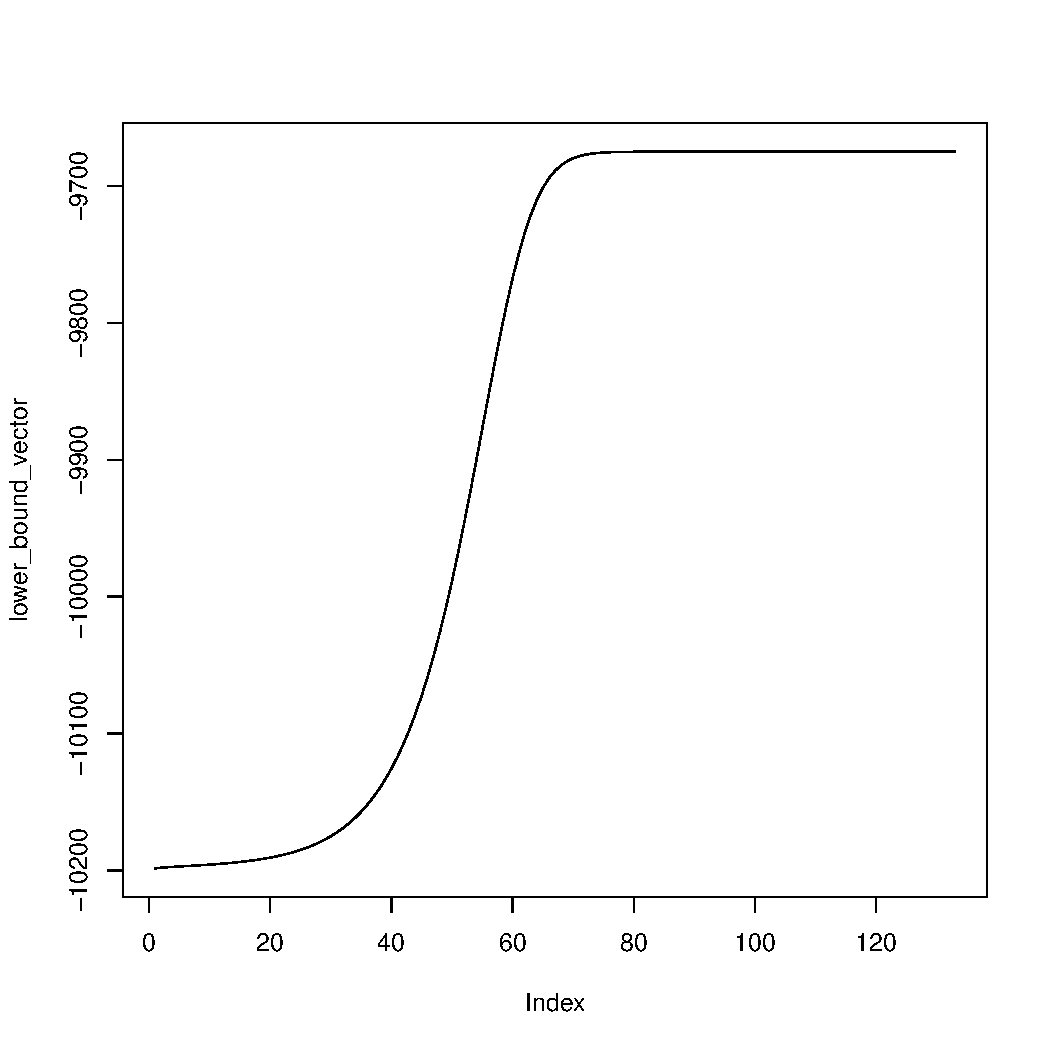
\includegraphics[width=100mm,height=100mm]{code/lower_bound_convergence.pdf}

\section{Extending the zero-inflated Poisson model to a regression model}
The above univariate model demonstrates that variational approximations are well-suited
to accelerating the fit of Bayesian zero-inflated models to data. Typically zero-inflated
models arise in applications where we wish to build multivariate regression models. To be able to
construct multivariate models with as much generality as possible, we specify the full
model as a General Design Bayesian Generalized Linear Mixed Model, as in \cite{zhao06}.
This allows us to incorporate within-subject correlation, measurement error, missing data
and smoothing splines in our models.

% TODO: Lower bound graph
% TODO: Accuracy of approximations
% TODO: Application, physical activity data
% Random intercept, longitudinal data
% Graph demonstrating additional zeroes

% Idea: We can use an approximation of the from q(\beta, \u, \Sigma) q(\rho) \Product q(r_i)
% and use GVA on q(\beta, \u, \Sigma) and mean field updates on \rho and r_i

\subsection{Model}
Let $\mR = \diag{(\vr)}$. Let $\mC = [X Z], \vnu = [\vbeta^T \vu^T]^T$.

$$
\begin{array}{rl}
\log{p(y|\vr, \vbeta, \vu)} &= \vy^T \mR (C\vnu) - \vr^T \exp{(C\vnu)} - \vone^T \log{\Gamma{(\vy + \vone)}}, \\
\log{p(\vnu|\sigma_{u}^2)} &= - \half \log{|2\pi \sigma_{\vu}^2 \mI|} - \half \vnu^T(\sigma_{\vu}^2 I)^{-1} \vnu, \\
\log{p(\vr)} &= \vr^T \log{(\rho \vone)} + (\vone - \vr)^T\log{(\vone - \vone \rho)}, \\
p(\rho) &\propto 1, \\
\mbox{and } \log{p(\sigma^2)} &= \alpha_{\sigma_\vu^2} \log{(\beta_{\sigma_\vu^2})} - \log{\Gamma{(\alpha_{\sigma_\vu^2})}} - (\alpha_{\sigma_\vu^2} + 1) \log{(\sigma_{\vu}^2)} - \frac{\beta_{\sigma_\vu^2}}{\sigma_{\vu}^2}\\
\end{array}
$$

\subsection{Approximation}
Let $r_0 = \{ r_i : y_i = 0 \}$.
We assume an approximation of the form
$$
q(r_0, \vnu, \sigma_{\vu}^2, \rho) = q(\vnu) q(\sigma_{\vu}^2) q(\rho) q(r_0) \\
$$

where

%\begin{align*}
$$
\begin{array}{rl}
q(\vnu) &= N(\vmu, \mLambda), \\
q(\sigma_{\vu}^2) &= IG\left(\alpha_{\sigma_u^2} + \frac{m}{2}, \beta_{\sigma_u^2} + \frac{\|\vmu_\vu\|^2}{2} + \frac{\tr(\mLambda_{\vu\vu})}{2}\right), \\
\mbox{and } q(r_i) &\propto \exp{\{\bE_{-r_i} [-r_i \exp{(c_i^T\vnu)}]\} + r_i [\psi(\alpha_\rho) - \psi(\beta_\rho)]}.\\
\end{array}
$$
%\end{align*}

Hence $q(r_i) = \Bernoulli{(p_i)}$ where
$$
p_i = \expit{\psi{(\alpha_{q(\rho)})} - \psi{(\beta_{q(\rho)})} - \exp{\{c_i^T\vnu + \half c_i^T \mLambda c_i\}}},
$$
where $i \in \{i : \vy_i = 0 \}$.

The optimal approximation for $\vr$ is
$$
\begin{array}{ll}
q(\vr) &\propto \exp{\{\bE_{-q(\vr)}y^T\mR(\mC\vmu) - \vr^T\exp{(\mC\vnu)}-\half \vnu^T \text{diag}(\sigma_{\vu}^2)^{-1} \vnu\}}
\end{array}
$$

$$
\begin{array}{ll}
&\bE_{-q(\vr)} [\vy^T\mR(C\vnu) - \vr^T\exp{(\mC\vnu)}-\half \vnu^T D(\sigma_{\vu}^2)^{-1} \vnu]\\
=&\vy^T\mR\mC \vmu - \vp^T \exp{\{\mC \vmu + \half \text{diag}(\mC \mLambda \mC^T)\}} - \half \vmu^T \hat{D} \vmu - \half \text{tr}(\mLambda \hat{D})
\end{array}
$$

where $\hat{\mD} = \frac{\alpha_{q(\sigma_{\vu}^2)}}{\beta_{q(\sigma_{\vu}^2)}} \mI$. This can be seen to be very close to a Poisson
regression model.

\subsection{Lower bound}
% Explain how most of the lower bound for the univariate model can simply be re-used, but \lambda is replaced
% with \vbeta, \vu
% You can build the lower bound out of re-usable terms like T_1, T_2, T_3, ...
% We're just introducing a replacement T_1
$$
\begin{array}{ll}
\bE_q [\log{p(y, \theta)} - \log{q(\theta)}] &= 
\vy \mP^T \mC \vmu - \vp^T\exp{(\mC\vmu + \half \vmu^T \mLambda \vmu)} - \vone^T\log{(\vy + \vone)}\\
&\quad + \half \log{|\mLambda|} + \frac{p + m}{2} (1 + \log{(2 \pi)})
\end{array}
$$

%For $\sigma^2_u$,
%$$
%\bE_q [\log{p(\sigma_u^2)} - \log{q(\sigma_u^2)}] = \frac{m}{2} \bE_q [\log{\sigma_u^{-2}}] - (\half \|\mu_u\|^2 + \tr(\Lambda_{uu})) \bE_q [\sigma_u^{-2}] - \log{\Gamma(\alpha_{\sigma_u^2})} + \log{\Gamma(\alpha_{\sigma_u^2} + \frac{m}{2} - 1)}
%$$
%
%where
%
%$$
%\bE_q[\log{(\sigma_u^2)}] = - \{\alpha_{\sigma_u^2}^2 - \log{\beta_{q(\sigma_u^2)}} + \log{\Gamma(\alpha_{q(\sigma_u^2)})} + (1-\alpha_{q(\sigma_u^2)})\psi{(\alpha_{q(\sigma_u^2)})}\}
%$$
%
%and
%
%$$
%\bE_q[\sigma_u^{-2}] = \frac{\alpha_{q(\sigma_u^2)}}{\beta_{q(\sigma_u^2)}}
%$$

For $\vnu$,

% Where are the priors for \vbeta and \vu

$$
\begin{array}{ll}
\bE_q[\log{p(\vnu)} - \log{q(\vnu)}] &= \vy^T \mP \mC \vmu - \vp^T \exp{(\mC \vmu + \half \vmu^T \mLambda \vmu)} - \vone^T\log \Gamma{(\vy + \vone)}\\
& \quad + \frac{p + m}{2} (1 + \log{2 \pi}) + \half \log{|\mLambda|}.
\end{array}
$$

% This should be denoted as T_3
For $\sigma^2_u$,
$$
\begin{array}{ll}
\bE_q[\log{p(\sigma^2_u)} - \log{q(\sigma^2_u)}] &=
\alpha_{\sigma^2_u} \log{\beta_{\sigma^2_u}} - \log{\Gamma{(\alpha_{\sigma^2_u})}} +
(\alpha_{\sigma^2_u} - 1) \bE_q	\log{\sigma^2_u}\\
&\quad - \beta_{\sigma^2_u} \bE_q [\sigma^2_u] +
\log{\Gamma(\alpha_{q(\sigma^2_u)})} - (\alpha_{q(\sigma^2_u)} - 1) \psi{(\alpha_{q(\sigma^2_u)})} - \log{(\beta_{q(\sigma^2_u)})}\\
&\quad - \log{(\alpha_{q(\sigma^2_u)} + \beta_{q(\sigma^2_u)})}\\
&=\alpha_{\sigma^2_u} \log{\beta_{\sigma^2_u}} - \log{\Gamma{(\alpha_{\sigma^2_u})}} +
(\alpha_{\sigma^2_u} - 1) \psi{\alpha_{q(\sigma^2_u)}} - \log{(\beta_{q(\sigma^2_u)})} \\
&\quad - \beta_{\sigma^2_u} \frac{\alpha_{q(\sigma^2_u)}}{\beta_{q(\sigma^2_u)}} + 
\log{\Gamma(\alpha_{q(\sigma^2_u)})} - (\alpha_{q(\sigma^2_u)} - 1) \psi{(\alpha_{q(\sigma^2_u)})} - \log{(\beta_{q(\sigma^2_u)})}\\
&\quad - \log{(\alpha_{q(\sigma^2_u)} + \beta_{q(\sigma^2_u)})}.
\end{array}
$$

where

$\alpha_{q(\sigma^2_u)} = \alpha_{\sigma^2_u} + m/2$ and
$\beta_{q(\sigma^2_u)} = \beta_{\sigma^2_u} + \|\vmu_\vu\|^2/2 +  \tr{(\mLambda_{\vu \vu})}/2$.

\subsection{Results}

\section{Theory of variational approximation of zero-inflated Poisson models}
Let $Z_i = R_i Y_i$.

Then the probability that $Z_i = 0$ is
$$
\begin{array}{rl}
P(Z_i = 0) &= P(R_i = 0)P(Y_i = y) + P(R_i = 1) P(Y_i = 0) - P(R_i = 0) P(Y_i = 0) \\
&= (1 - \rho) + \rho e^{-\lambda} - (1 - \rho) e^{-\lambda} \\
&= (1 - \rho) + e^{-\lambda}(2 \rho - 1)
\end{array}
$$

\section{Appendix - Algebraic derivations of conditional likelihoods}

The joint likelihood is:

$$
p(\vx, \vr, \lambda, \rho) = \frac{b^a \lambda^{a - 1} \exp{(-b \lambda)}}{\Gamma{(a)}} \prod_{i=1}^n \frac{\exp{(-\lambda r_i)} (\lambda r_i)^{x_i}}{x_i !} \rho^{r_i} (1 - \rho)^{1 - r_i}.
$$

%\begin{align*}
%p(\lambda|\vx, \vr, \rho) &= \frac{\prod_{i=1}^n p(x_i | \lambda, r_i) p(\lambda) p(r_i|\rho) p(\rho)}{\int \prod_{i=1}^n p(x_i | \lambda, r_i) p(\lambda) p(r_i|\rho) p(\rho)) d \lambda}.
%\end{align*}
%
%Concentrating for now on the denominator in this expression, we re-arrange and collect
%like terms to obtain
%$$
%\prod_{i=1}^n \rho^r_i (1 - \rho)^{1 - r_i} \frac{r_i^{x_i}}{x_i !}
%	\int \frac{b^a \lambda^{a - 1} \exp{(-b \lambda)} \lambda^{x_i} \exp{(-\lambda r_i)}}{\Gamma{(a)}} d \lambda
%$$
%
%The integral in this expression is
%\begin{align*}
%& \int \frac{b^a \lambda^{(a + x_i) - 1} \exp{(-\lambda(b + r_i))}}{\Gamma{(a + x_i)}} d \lambda \frac{\Gamma{(a+ x_i)}}{\Gamma{(a)} b^{-x_i}} \\
%=& \frac{\Gamma{(a+ x_i)}}{\Gamma{(a)} b^{-x_i}}.
%\end{align*}
%
%Collecting the multiplicands in the integral over $\lambda$ together, we obtain
%$$
%\prod_{i=1}^n \rho^{r_i} (1 - \rho)^{1 - r_i} \frac{r_i^{x_i}}{x_i!}
%	\int \frac{b^{na + \sum_{i=1}^n x_i} \lambda^{(na + \sum_{i=1}^n x_i) - 1} \exp{(-\lambda(nb + \sum_{i=1}^n r_i))}}{\Gamma{(na + \sum_{i=1}^n x_i)}} d \lambda
%	\frac{\Gamma{(na + \sum_{i=1}^n x_i)}}{\Gamma{(na)} b^{-\sum_{i=1}^n x_i}}.
%$$

%By cancelling like terms in the numerator and denominator of the full likelihood we arrive 
%at

$$
\beta_{\lambda}^{\alpha_\lambda+\vone^T\vx} \lambda^{(\alpha_\lambda + \vone^T\vx) - 1} \exp{\left(-(\beta_\lambda + \vone^T\vr) \lambda \right)}
$$

$$
\frac{\rho^{\vone^T\vr} (1 - \rho)^{\vone^T(\vone - \vr)}}{\Beta{\alpha_\rho + \vone^T \vr, \beta_\rho + \vone^T(\vone - \vr)}}
$$

$$
\begin{array}{ll}
p(r_i | \text{rest}) &\propto \frac{(\lambda r_i)^{x_i} \exp{(-\lambda r_i)}}{x_i !} \rho^{r_i} (1 - \rho)^{1 - r_i} \\
&\propto r_i^{x_i} (e^{-\lambda})^{r_i} \rho^{r_i} (1 - \rho)^{1 - r_i}
\end{array}
$$

We make use of the fact that if $x_i = 0$, $r_i = 0$, and if $x_i \ne 0$,
$r_i = 1$. So $x_i^{r_i} = I(x \ne 0)$ and hence the likelihood can be re-written as

$$
\begin{array}{ll}
p(r_i | \text{rest}) &= \frac{(e^{-\lambda + \logit{(\rho)}})^{r_i}}{I(x_i = 0) + (e^{-\lambda + \logit{(\rho)}})^{r_i}}
\end{array}
$$

\bibliographystyle{plain}
\bibliography{Chapter_1_zero_inflated_models}

\end{document}
